\documentclass[12pt,a4paper]{article}

%% moduł ustawiający geometrię dokumentu w sposób optymalny dla raportu projektowego, przede
%% wszystkim marginesy sekcji ustawione zostają na standardowy 1 cal.
\usepackage[margin=1.0in,nomarginpar]{geometry}

%% moduł umozliwiający pisanie dokumentów w języku polskim (kodowanie UTF-8) i zamieniający 
%% język opisu najważniejszych obiektów w dokumencie (rozdział, spis treści, itp.)
\usepackage{polski}
\usepackage[utf8]{inputenc}

%% moduł umożliwiający wstawianie grafik do dokumentu
\usepackage{graphicx}
\graphicspath{ {figures/} } % wszystkie grafiki w dokumencie należy umieszczać w podfolderze 'figures'

%% moduł, który dodaje wcięcie w pierwszym akapicie każdej rozpoczynanej sekcji
\usepackage{indentfirst}  

%% moduły umożliwające stosowanie symboli i równań matematycznych
\usepackage{amssymb}
\usepackage{amsmath}
\usepackage{textcomp}
\usepackage{gensymb}

%% moduł umożliwiający stosowanie list numerowanych
\usepackage{enumerate}



%% Nagłówek dokumentu
%% ----------------------------------------------------------------------------------------------------

\begin{document}

\title{Pompy i Transformatory Ciepła ESN0822P - Projekt} % należy podać nazwę i kod zajęć projektowych
\author{Jan Kowalski, Katarzyna Malinowska \\ % należy wpisać jedno lub kilka imion i nazwisk oddzielając przecinkami
	\\
	Wydział Mechaniczno-Energetyczny, Politechnika Wrocławska \\
	2017/2018, semestr zimowy
	}

\maketitle

%% wyświetlenie spisu treści wygenerowanego automatycznie na podstawie zawartości całego dokumentu
\tableofcontents



%% Zawartość poszczególnych rozdziałów, sekcji i akapitów
%% ----------------------------------------------------------------------------------------------------

\chapter{Wprowadzenie}

\section{Wstęp}
Lorem ipsum dolor sit amet, consectetur adipiscing elit. Nunc molestie orci vel elit vehicula tempor. Duis a ipsum iaculis, aliquet libero eget, fringilla tortor. Etiam bibendum viverra suscipit. Pellentesque bibendum erat venenatis lacus placerat iaculis. Quisque id varius urna. In malesuada orci id risus vulputate semper. Proin ac aliquam erat, id pellentesque erat. Quisque aliquet eu orci a tempor. Nunc maximus hendrerit iaculis. Praesent tincidunt lorem nunc, vel cursus velit iaculis vehicula. Quisque non dictum augue. Proin sagittis nisl a dolor tincidunt, convallis lobortis purus bibendum. Proin vitae consectetur augue, vitae pulvinar nunc. Suspendisse luctus sed ex vitae cursus. Curabitur lacinia felis vel ligula feugiat laoreet. Nunc sed nisi a urna venenatis dapibus id ac nisl.

Nunc vitae posuere leo. Sed tempus quis tortor pretium aliquam. Mauris vehicula eleifend tellus et accumsan. Ut blandit pretium rhoncus. Sed nec lobortis lacus. Vivamus dapibus mauris non commodo aliquet. In facilisis pellentesque neque eget bibendum. Phasellus ornare odio est, id venenatis lacus gravida ac. Sed ac eros sed est rutrum aliquam in ac nisl. Sed sagittis fringilla nisi at mollis.



\subsection{Wybór rodzaju przechowywanego materiału medycznego}
Sposób przechowywania preparatów biologicznych powinien zapewniać spowolnienie przemian metabolicznych i utraty związków energetycznych. Możliwe jest to poprzez odpowiednie schłodzenie tkanek (wprowadzenie ich w stan hipotermii). 
Wyróżnia się różne rodzaje preparatów medycznych, które wymagają przechowywania w niskiej temperaturze \cite{Volmer2016}. Mogą to być:

\begin{itemize}

	\item Curabitur tellus nisl, faucibus a finibus id, interdum id nisl. Maecenas suscipit, ex non pharetra varius, arcu nulla tincidunt metus, in euismod quam sem nec est. Duis gravida turpis at ligula rutrum, sed scelerisque ipsum iaculis. Curabitur laoreet magna vel nibh ultrices, quis dictum nibh aliquam \cite{Biala2012}.
	
	\item ivamus rutrum justo turpis, quis eleifend tortor malesuada non. Proin a nibh risus. Suspendisse malesuada enim tristique tellus pretium, quis molestie ante fringilla. Phasellus ut justo varius, venenatis ipsum in, interdum ligula. Interdum et malesuada fames ac ante ipsum primis in faucibus.  
	
	\item Nulla rhoncus vehicula tortor, eget semper erat tempor id. Nulla facilisi. Quisque malesuada pharetra neque, nec eleifend dolor consequat non. Donec tempus risus nec dui cursus, quis dapibus odio pulvinar. Suspendisse aliquet enim vel lacus hendrerit eleifend. Mauris et nisl sed diam eleifend maximus nec sed risus. Quisque elementum neque sed semper rutrum. Integer ut ullamcorper quam. 

\end{itemize}

Nulla congue ultrices erat, nec pretium sem tristique sed. Cras at imperdiet augue. Nulla non malesuada nunc. Donec commodo nisi ac facilisis volutpat. Proin pretium porta ante, ut blandit dolor molestie ut. Aliquam tristique faucibus egestas. In euismod tempor sem, at dapibus lectus placerat et. Przykład rozwiązania przedstawiono na rys. \ref{fig:sample}.

\begin{figure}[!ht]
	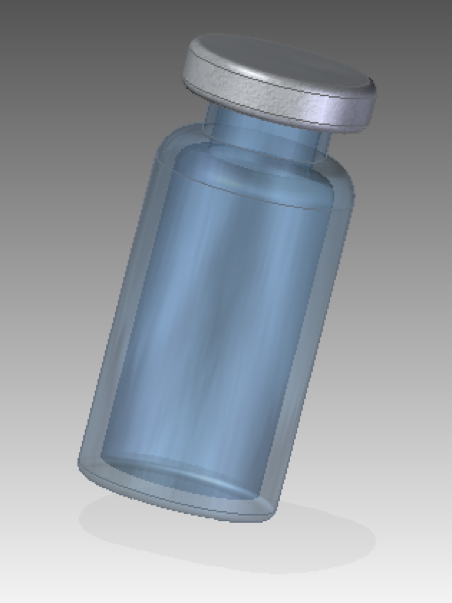
\includegraphics[width=0.4\textwidth]{sample}
	\centering
	\caption{Nulla congue ultrices erat.}
	\label{fig:sample}
\end{figure}

Duis et volutpat leo. Sed eget porta sapien. Quisque purus sem, posuere non mi quis, ullamcorper aliquam nulla. Fusce cursus dui a urna pharetra, id tempus lectus consectetur. Donec varius rhoncus tortor eget aliquam. Aliquam malesuada nibh quis nunc pulvinar, vel malesuada enim pellentesque. Proin maximus ullamcorper quam, a sodales elit bibendum eget. Mauris pellentesque, metus vitae elementum eleifend, lorem odio luctus leo, pretium auctor velit risus in sem. Morbi vel elit aliquet massa eleifend rutrum et at odio. Nulla commodo lacus a ultricies posuere. Praesent dapibus pulvinar diam ac ornare. Vestibulum ut sollicitudin neque. Morbi lacinia lobortis egestas. Phasellus semper lorem a tellus scelerisque lacinia. Maecenas blandit facilisis eros, dignissim commodo lacus tristique eget.

Proin euismod ipsum in enim facilisis fringilla. Duis ac metus accumsan, tristique ligula at, molestie lectus. Ut feugiat nibh et leo gravida accumsan. Donec lorem nisi, imperdiet non porta vitae, dictum vitae metus. Donec aliquam tincidunt risus sed fermentum. Suspendisse dapibus tortor orci, vel ultricies ex mollis et. Praesent molestie rhoncus enim, quis consequat turpis consequat eget. Curabitur commodo nisl at elementum ullamcorper. Aenean venenatis sodales nisl, at feugiat neque dapibus quis. Praesent sollicitudin ligula non nisl blandit viverra. Ut eu pulvinar mauris.

\subsection{Prawidłowe przechowywanie szczepionek}
In posuere, turpis a mollis ultricies, augue nunc porttitor sapien, sed accumsan lectus nibh ultrices risus. Vestibulum eget lectus id ipsum efficitur tristique. Mauris sit amet risus dolor. Pellentesque nulla erat, tempus quis ultricies quis, ultricies eu risus. Phasellus mattis mauris eu urna semper, euismod vulputate libero pharetra. Morbi sit amet augue nec sem faucibus aliquam imperdiet id erat. Sed facilisis arcu sed ipsum sollicitudin, vitae condimentum arcu blandit. Curabitur ex nulla, ultricies non dui in, porta sollicitudin felis. Quisque sit amet dignissim tortor, a tristique lorem. In luctus magna vitae vestibulum condimentum. Nullam tristique eget eros et consectetur. Phasellus lobortis laoreet vulputate. Donec dapibus at nulla et dignissim. Phasellus vehicula mauris vitae elit sodales, nec semper mi vestibulum \cite{Volmer2016}.



Phasellus vehicula vel libero quis lobortis. Pellentesque luctus ligula in arcu sagittis, sit amet dapibus velit pretium. Orci varius natoque penatibus et magnis dis parturient montes, nascetur ridiculus mus. Donec nisl velit, ultrices at nulla ac, porta malesuada ipsum. Praesent at ligula gravida, eleifend eros pulvinar, iaculis ipsum. Mauris non risus auctor, pharetra enim vel, vestibulum libero. Pellentesque porta a tortor at aliquam. Etiam vel elit ligula. In accumsan purus massa, a imperdiet lacus viverra quis. Class aptent taciti sociosqu ad litora torquent per conubia nostra, per inceptos himenaeos.

Pellentesque a eros lobortis, sodales urna a, fringilla nisi. Vestibulum gravida purus non tempus hendrerit. Orci varius natoque penatibus et magnis dis parturient montes, nascetur ridiculus mus. Sed molestie est arcu, auctor venenatis tellus euismod vitae. Nunc porttitor hendrerit purus, ut volutpat libero accumsan at. Maecenas mauris ipsum, dignissim non fringilla quis, bibendum id turpis. Sed scelerisque mi nec sapien consectetur, non bibendum arcu aliquam. Interdum et malesuada fames ac ante ipsum primis in faucibus. Proin faucibus scelerisque felis, eget rutrum ex consectetur quis. Nullam id euismod risus. Nunc a risus aliquet, lacinia tellus ut, porttitor ante. Orci varius natoque penatibus et magnis dis parturient montes, nascetur ridiculus mus. Pellentesque convallis euismod ex, eu pulvinar est pharetra sit amet. Suspendisse at aliquet mauris. Phasellus neque arcu, pretium eu ante et, hendrerit dignissim tellus \cite{Smith2012}. 




\chapter{Obliczenia projektowe}

\section{Obliczenia i wzory}

\subsection{Przemiana politropowa}
Dla przemiany politropowej prawdziwa jest zależność:

\begin{equation}
p \cdot V^n = idem
\label{eq:number_4}
\end{equation}

Aby wyeliminować objętość należy spierwiastkować równanie \eqref{eq:number_4}, co prowadzi do postaci:

\[p^{\frac {1}{n}} \cdot V = idem\]

Równanie Clapeyrona przekształcone celem uzyskania objętości po lewej stronie ma postać:

\[V = \frac{nRT} {p}\]

Zestawiając obie równości uzyskuje się:

\[p^{\frac {1}{n}} \cdot \frac{nRT} {p} = idem\]

Po podzieleniu obu stron równania przez $nR$ (stała) oraz zapisaniu $1/p$ jako $p^{-1}$ równanie przyjmuje postać:

\[p^{\frac {1}{n}} \cdot p^{-1} \cdot T = idem\]

Ponieważ $x^a \cdot x^b = x^{a+b}$ uporządkowanie powyższego równania prowadzi ostatecznie do zależności pomiędzy temperaturą i ciśnieniem przemiany politropowej:

\[p^{\frac {1-n}{n}} \cdot T = idem\]

Zakładając, że przemiana politropowa przebiega pomiędzy stanami 1 i 2, można zapisać następującą równość:

\[p_1 ^{\frac {1-n}{n}} \cdot T_1 = p_2 ^{\frac {1-n}{n}} \cdot T_2\]

Co daje się uporządkować do następujących postaci:

\begin{equation}
\frac{T_1}{T_2} =   \left( \frac {p_2}{p_1}\right) ^{\frac {1-n}{n}}
\label{eq:number_5}
\end{equation}

\begin{equation}
\frac{p_2}{p_1} =   \left( \frac {T_2}{T_1}\right) ^{\frac {n}{n-1}}
\label{eq:number_6}
\end{equation}


\subsection{Obliczenie wykładnika przemiany }
Aby możliwe było obliczenie wykładnika przemiany, konieczne jest przekształcenie równania \eqref{eq:number_5}. Zlogarytmowanie obu stron równania prowadzi do następującej postaci:

\[log \left( \frac{T_1}{T_2} \right) = log \left( \frac{p_2}{p_1} \right)^ {\left( \frac{1-n}{n} \right)} \]

Ponieważ $log(a)^b = b\cdot log(a)$:

\[log \left( \frac{T_1}{T_2} \right) = \left( \frac{1-n}{n} \right) \cdot log \left( \frac{p_2}{p_1} \right)\]

Po pomnożeniu obu stron przez $n$:

\[n \cdot log \left( \frac{T_1}{T_2} \right) = \left( {1-n} \right) \cdot log \left( \frac{p_2}{p_1} \right)\]

Wykonujemy mnożenie po prawej stronie:

\[n \cdot log \left( \frac{T_1}{T_2} \right) = log \left( \frac{p_2}{p_1} \right) - n \cdot log \left( \frac{p_2}{p_1} \right)\]

Przenosimy iloczyn przez $n$ na lewą stronę i wyciągamy $n$ przed nawias:

\[n \cdot \left[ log \left( \frac{T_1}{T_2} \right) + log \left( \frac{p_2}{p_1} \right) \right] = log \left( \frac{p_2}{p_1} \right)\]

Sumę logarytmów można zapisać jako logarytm iloczynu:

\[n \cdot \left[ log \left( \frac{T_1}{T_2} \cdot \frac{p_2}{p_1} \right) \right] = log \left( \frac{p_2}{p_1} \right)\]

Ostatecznie wykładnik politropy oblicza się z następującej zależności:

\[n = \frac {log \left( \frac{p_2}{p_1} \right)} {log \left( \frac{T_1}{T_2} \cdot \frac{p_2}{p_1} \right)}  \]



\subsection{Praca przemiany politropowej}
W termodynamice pracę $L_{1-2}$ oblicza się całkując:

\begin{equation}
L_{1-2} = \int_1^2 p\cdot dV
\label{eq:number_7}
\end{equation}


Wiedząc, że dla przemiany politropowej obowiązuje równanie \eqref{eq:number_4} można zapisać:

\begin{equation}
p = \frac{idem}{V^n}
\label{eq:number_8}
\end{equation}
Co po podstawieniu do równania \eqref{eq:number_7} daje:

\[L_{1-2} = \int_1^2 {\frac{idem}{V^n} \cdot dV} \]

Po uporządkowaniu:

\[L_{1-2} = idem \cdot \int_1^2 V^{-n} \cdot dV \]

Pamiętając, że $\int x^a = \frac{x^{a+1}}{a+1} + C$ rozwiązujemy całkę otrzymując:

\[L_{1-2} = idem \cdot \left( \frac{V_2 ^{1-n}}{1-n} - \frac{V_1 ^{1-n}}{1-n} \right)\]

Po uporządkowaniu:

\[L_{1-2} = \frac{idem}{1-n} \cdot \left( V_2 ^{1-n} - V_1 ^{1-n} \right)\]

Uwzględniając, że $x^{1-a} = x^1 \cdot x^{-a}$ możemy zapisać:

\[L_{1-2} = \frac{idem}{1-n} \cdot \left( V_2 \cdot V_2^{-n} - V_1 \cdot V_1^{-n} \right)\]

Uporządkowując zapis do postaci...

\[L_{1-2} = \frac{1}{1-n} \cdot \left( V_2 \cdot \frac {idem}{V_2^{n}} - V_1 \cdot \frac{idem}{V_1^{n}} \right)\]

Oraz podstawiając równanie \eqref{eq:number_8} rówanie przyjmuje postać:

\[L_{1-2} = \frac{1}{1-n} \cdot \left( p_2 \cdot V_2 - p_1 \cdot V_1 \right)\]

Co po wyciągnięciu z nawiasu $-1$ daje ostatecznie równanie na pracę przemiany politropowej:

\[L_{1-2} = \frac{1}{n-1} \cdot \left( p_1 \cdot V_1 - p_2 \cdot V_2 \right)\]

Podstawiając odpowiednie wartości z zadania uzyskuje się:

\[L_{1-2} = \frac{1}{n-1} \cdot \left( p_1 \cdot V_1 - p_2 \cdot V_2 \right)\]

Niestety do rozwiązania wciąż brakuje nam informacji o objętości w stanie 2. Na szczęście można ją wyeliminować. W tym celu należy zapisać równanie politropy dla dwóch stanów 1 i 2. 

\[ p_1 \cdot V_1 ^n = p_2 \cdot V_2 ^n \]

Przekształcając:

\[\frac{p_2}{p_1} = \frac{V_1 ^n}{V_2 ^n} \]

Pierwiastkując w stopniu $n$:

\[\left( \frac{p_2}{p_1} \right) ^{\frac{1}{n}} = \frac{V_1}{V_2} \]

\[V_2 = V_1 \cdot \left( \frac{p_2}{p_1} \right) ^{-\frac{1}{n}} \]

Podstawiając do równania na pracę:

\[L_{1-2} = \frac{1}{n-1} \cdot \left( p_1 \cdot V_1 - p_2 \cdot V_1 \cdot \left( \frac{p_2}{p_1} \right) ^{-\frac{1}{n}}  \right)\]

Teraz można wyciągnąć $p_1 \cdot V_1$ przed nawias:

\[L_{1-2} = \frac{1}{n-1} \cdot  p_1 \cdot V_1\cdot \left(1 - V_1 \cdot \frac{p_2}{p_1} \cdot  \left( \frac{p_2}{p_1} \right) ^{-\frac{1}{n}}  \right)\]

Ostatecznie uzyskuje się równanie na pracę przemiany politropowej, do rozwiązania którego nie jest potrzebna znajomość objętości na końcu:

\[L_{1-2} = \frac{1}{n-1} \cdot  p_1 \cdot V_1\cdot \left(1 - \left( \frac{p_2}{p_1} \right) ^{\frac{n-1}{n}}  \right)\]


%\appendix
%\include{appendixa}
%\include{appendixb}


%% Zawartość poszczególnych rozdziałów, sekcji i akapitów
%% ----------------------------------------------------------------------------------------------------

%% Wskazanie pliku z bibliografią (bibliography.bib) oraz stylu w jakim będzie wyświetlana lista źródeł.

\bibliography{bibliography}
\bibliographystyle{plain}


\end{document}

